\documentclass[a4paper,12pt]{article}
\usepackage{times}
\usepackage[francais]{babel}
\usepackage[utf8]{inputenc}
\usepackage[T1]{fontenc}
\usepackage{amsmath}
\usepackage{amssymb}
\usepackage{graphicx}
\usepackage{pdfpages}
\usepackage{pdflscape}
\usepackage{listings}
\usepackage{longtable}
\usepackage{hyperref}
\lstset{literate=
{é}{{\'e}}1
{è}{{\`e}}1
{ê}{{\^e}}1
{à}{{\`a}}1
{â}{{\^a}}1
}
\lstset{language=C++,
                basicstyle=\footnotesize,
                keywordstyle=\footnotesize\color{blue},
                otherkeywords={override,nullptr}
}
\definecolor{orange}{rgb}{0.8,0.4,0.0}
\definecolor{darkblue}{rgb}{0.0,0.0,0.6}
\definecolor{cyan}{rgb}{0.0,0.6,0.6}
\lstdefinelanguage{JSON}
{
  basicstyle=\normalsize,
  columns=fullflexible,
  showstringspaces=false,
  commentstyle=\color{gray}\upshape,
  morestring=[b]",
  morestring=[s]{>}{<},
  morecomment=[s]{<?}{?>},
  stringstyle=\color{orange},
  identifierstyle=\color{darkblue},
  keywordstyle=\color{blue},
  morekeywords={string,number,array,object}% list your attributes here
}

\sloppy

\setlength{\topmargin}{0cm}
\setlength{\headsep}{0.in}
\setlength{\headheight}{0.in}
\setlength{\evensidemargin}{0cm}
\setlength{\oddsidemargin}{-1cm}
\textwidth 18cm
\textheight 25cm

\begin{document}

\thispagestyle{empty}

\begin{titlepage}

\vspace*{2cm}

\begin{center}\textbf{\Huge Projet Logiciel Transversal}\end{center}{\Large \par}

\begin{center}\textbf{\large Alexandre Génot - Anthony Peloille}\end{center}{\large \par}

\vspace{2cm}

\begin{figure}[h]
\begin{center}
\includegraphics[width=\textwidth]{slaythespire.jpg}
\caption{\label{Slay the Spire}Slay the Spire}
\end{center}
\end{figure}

\clearpage

{\small
\tableofcontents
}

\end{titlepage}

\clearpage
\section{Présentation Générale}

\subsection{Archétype}

Les mécaniques du jeu s'inspirent de Slay the Spire (2017) qui est un rogue-like avec un système de combat basé sur l'utilisation de cartes.

\subsection{Règles du jeu}

Le joueur évolue dans un donjon dont la structure des étages est générée aléatoirement. A chaque étage il doit atteindre un boss, pour cela il se déplace de case en case à la manière d’un jeu de plateau. Chaque case contient un évènement (il y a différents types d’évènements : combat, magasin, récompense, bonus ou malus). Le but est de sortir du donjon en ayant complété chaque étage (avoir vaincu tous les boss). Le système de combat est basé sur l’utilisation de cartes permettant au joueur d’affronter ses adversaires (le nombre d’adversaires augmente au cours du jeu). Les cartes sont obtenues en récompenses de combat, au magasin ou lors d’évènements aléatoires. Le personnage peut trouver de l’équipement lui permettant d’augmenter ses statistiques (vie, armure, puissance).

\subsection{Ressources}

\begin{figure}[h]
\begin{center}
\includegraphics[width=0.5\textwidth]{dungeontile.png}
\caption{\label{tiles}Tuiles du décor et personnages}
\end{center}
\end{figure}

\begin{figure}[h]
\begin{center}
\includegraphics[width=0.5\textwidth]{card.png}
\caption{\label{card}Template de carte utilisé lors des combats}
\end{center}
\end{figure}

\begin{figure}[h]
\begin{center}
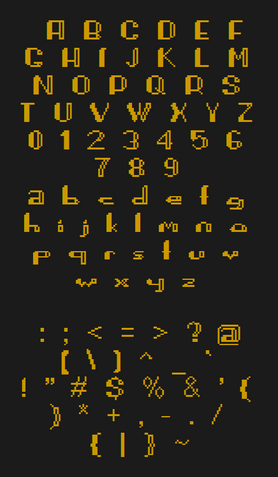
\includegraphics[width=0.5\textwidth]{font.png}
\caption{\label{font}Police de caractères}
\end{center}
\end{figure}

\clearpage
%\section{Description et conception des états}
%
%\subsection{Description des états}
%
%
%\subsection{Conception Logiciel}
%
%
%%\begin{landscape}
%%\begin{figure}[p]
%%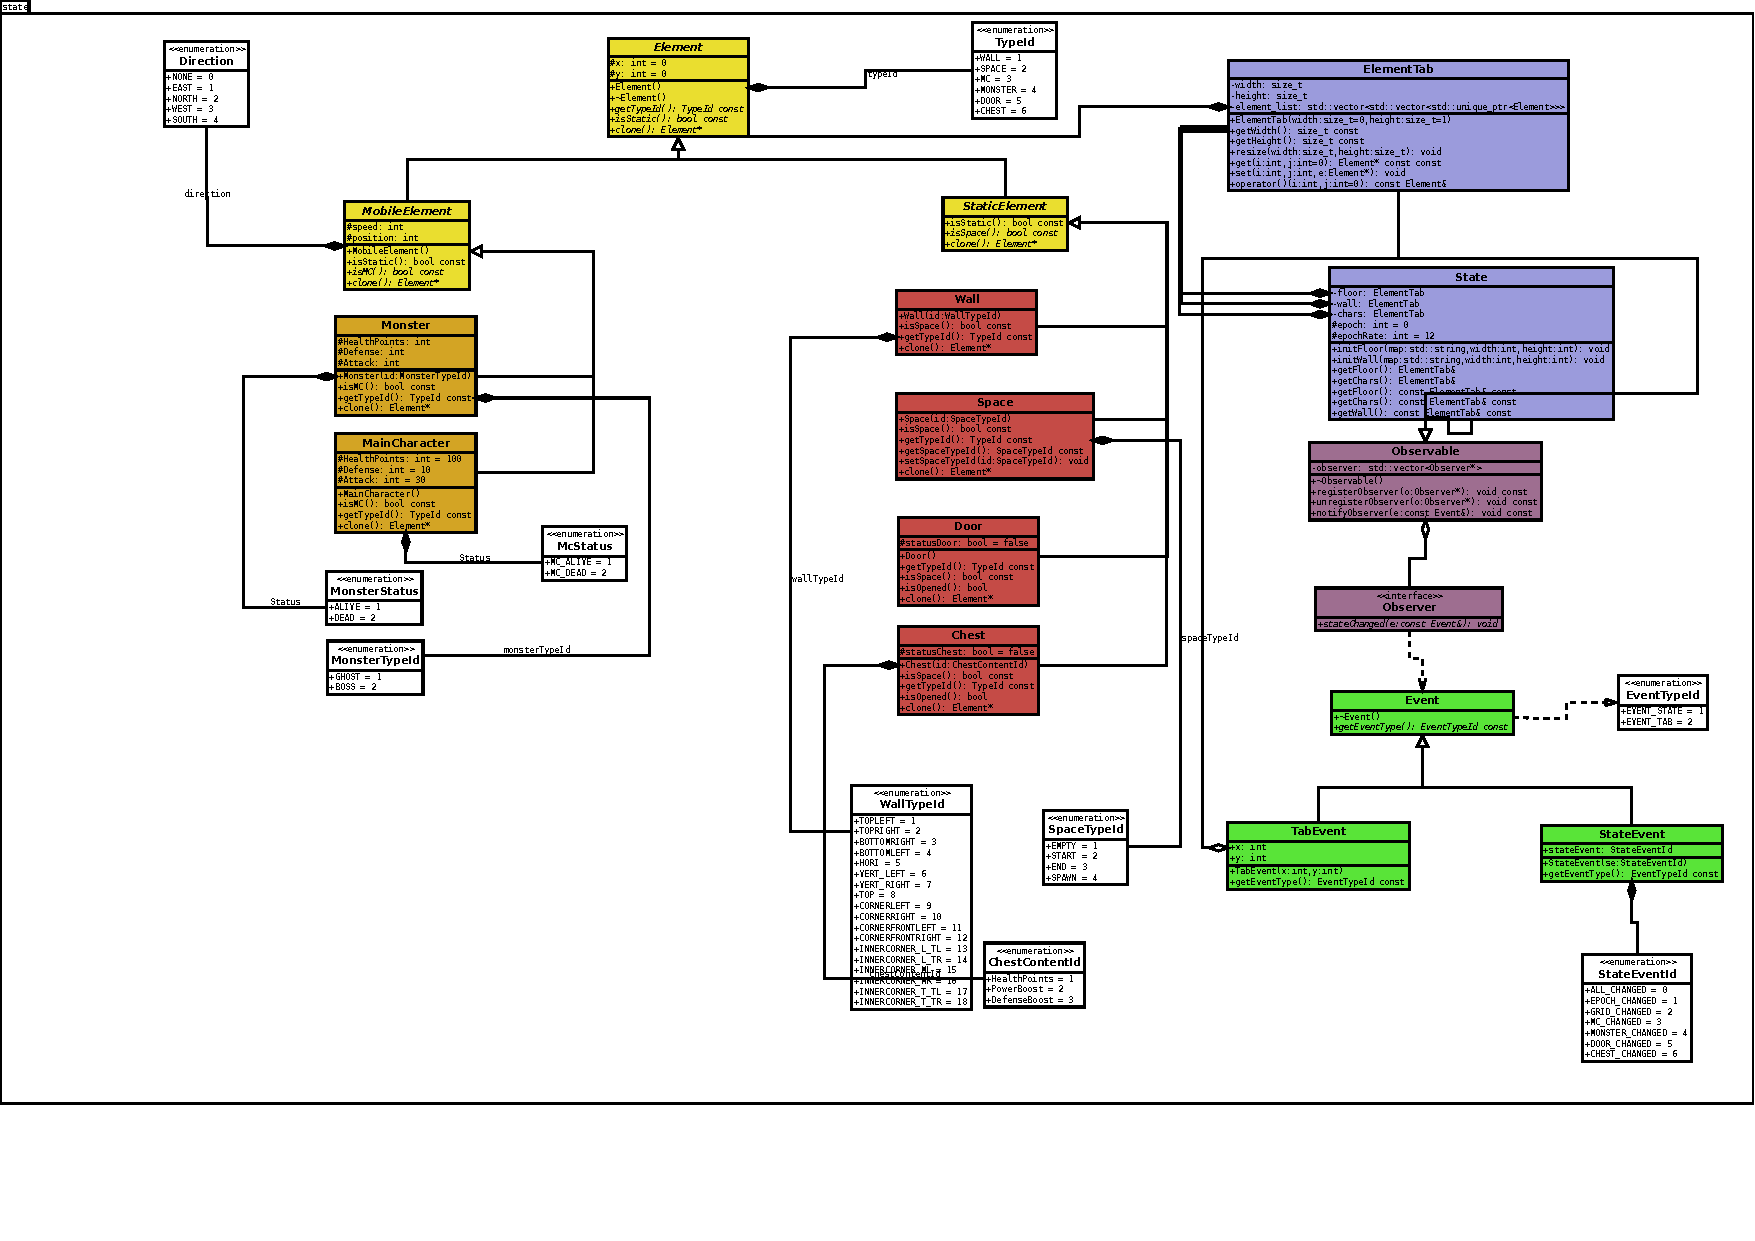
\includegraphics[width=0.9\paperheight]{state.pdf}
%%\caption{\label{uml:state}Diagramme des classes d'état.} 
%%\end{figure}
%%\end{landscape}
%
%\clearpage
%\section{Rendu: Stratégie et Conception}
%
%\subsection{Stratégie de rendu d'un état}
%
%
%\subsection{Conception logiciel}
%
%%\begin{landscape}
%%\begin{figure}[p]
%%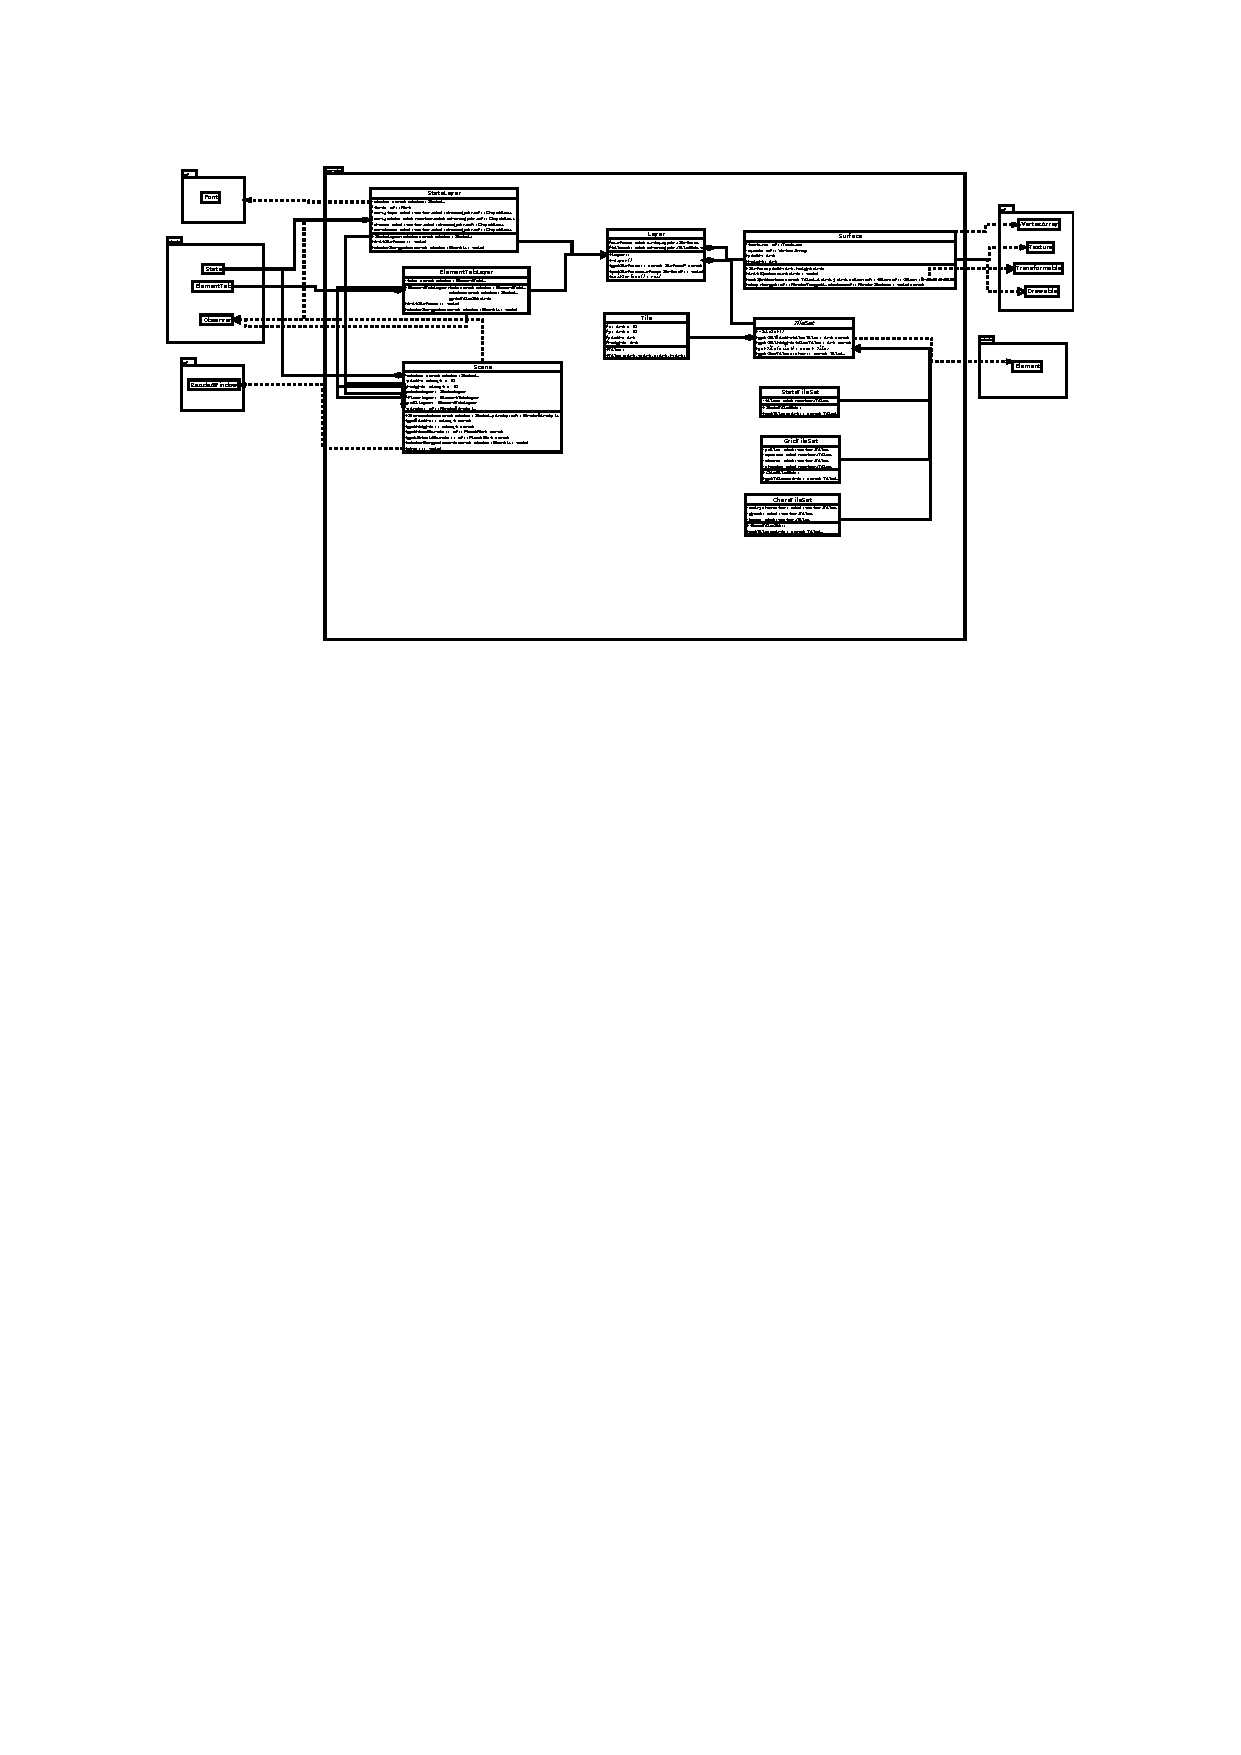
\includegraphics[width=0.9\paperheight]{render.pdf}
%%\caption{\label{uml:render}Diagramme des classes de rendu.} 
%%\end{figure}
%%\end{landscape}
%
%\clearpage
%\section{Règles de changement d'états et moteur de jeu}
%
%\subsection{Règles}
%
%\clearpage
%\subsection{Conception logiciel}
%
%
%%\begin{landscape}
%%\begin{figure}[p]
%%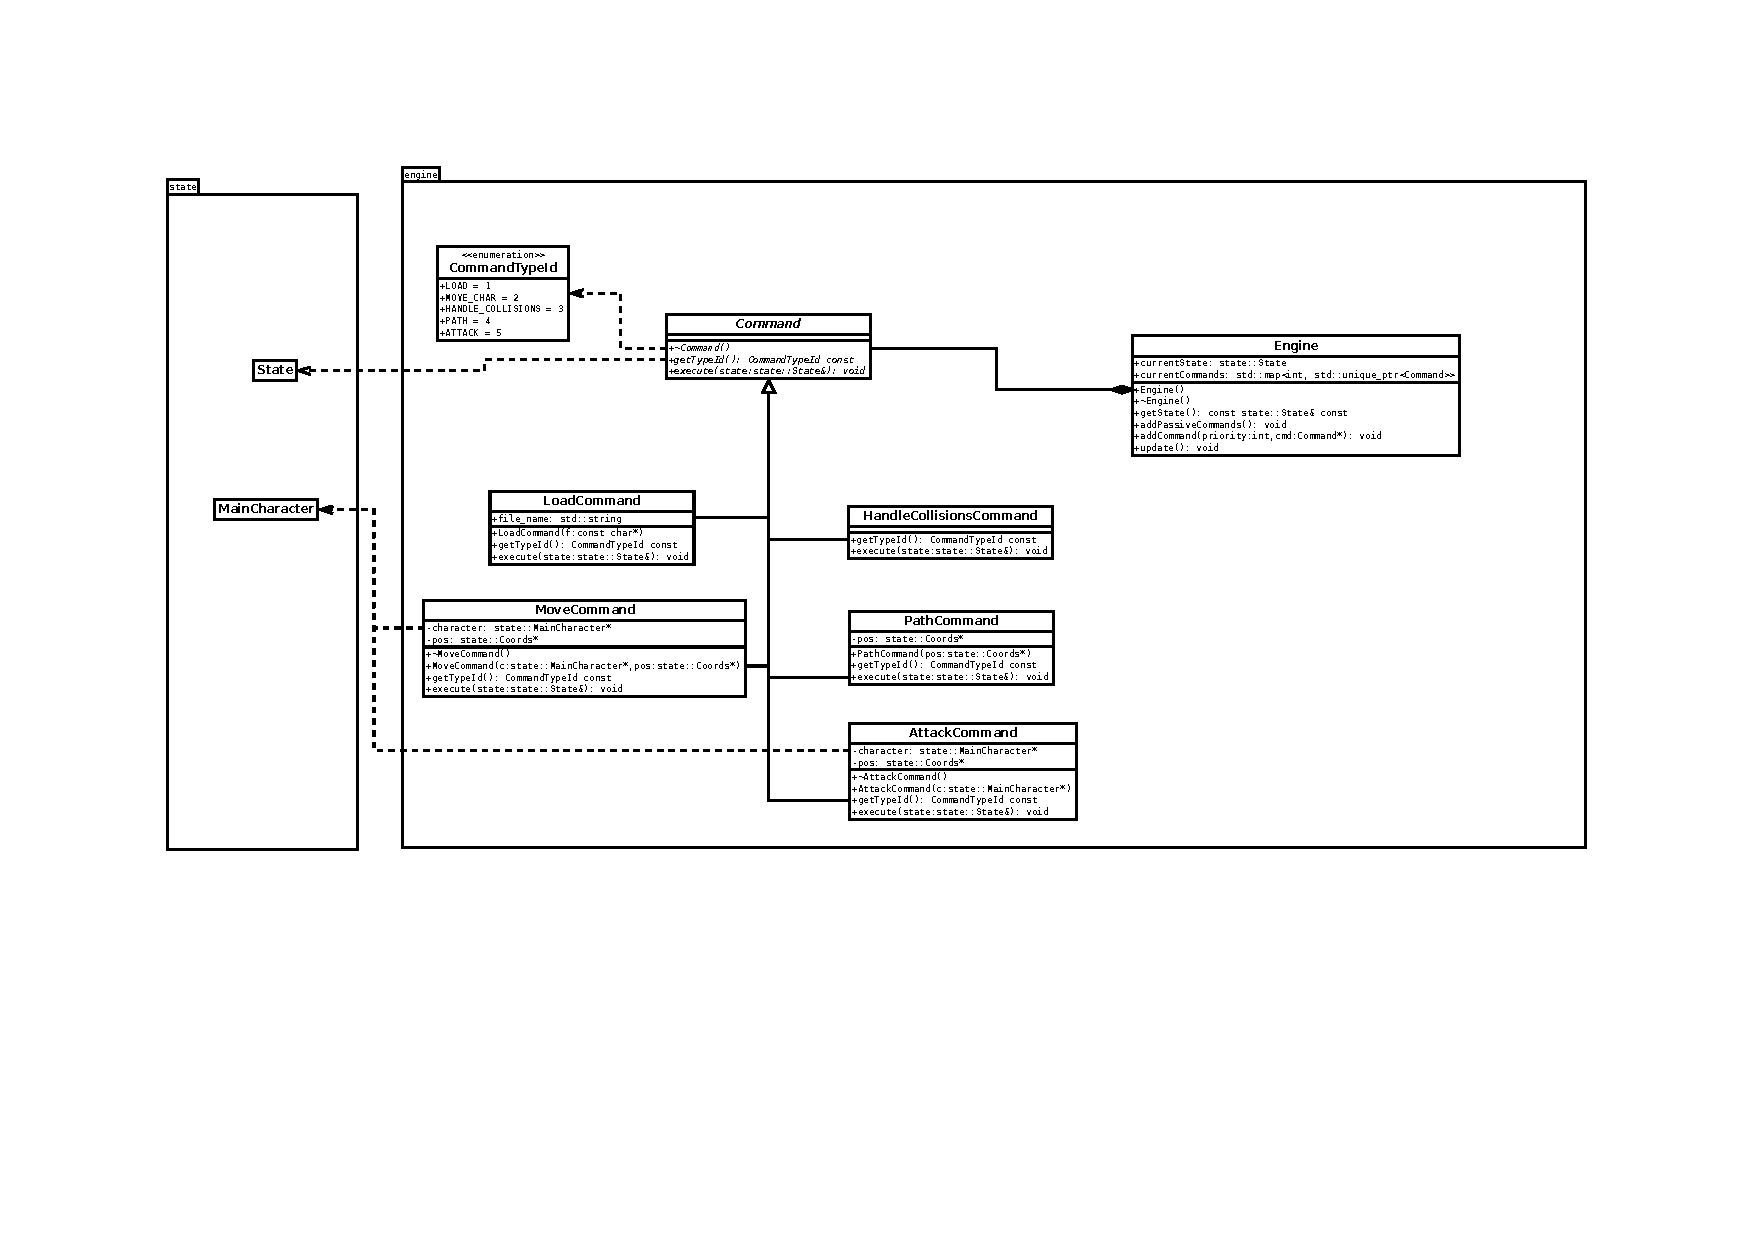
\includegraphics[width=0.9\paperheight]{engine.pdf}
%%\caption{\label{uml:engine}Diagramme des classes de moteur de jeu.} 
%%\end{figure}
%%\end{landscape}
%
%
%\section{Intelligence Artificielle}
%
%\subsection{Stratégies}
%
%\clearpage
%\subsection{Conception logiciel}
%
%
%%\begin{landscape}
%%\begin{figure}[p]
%%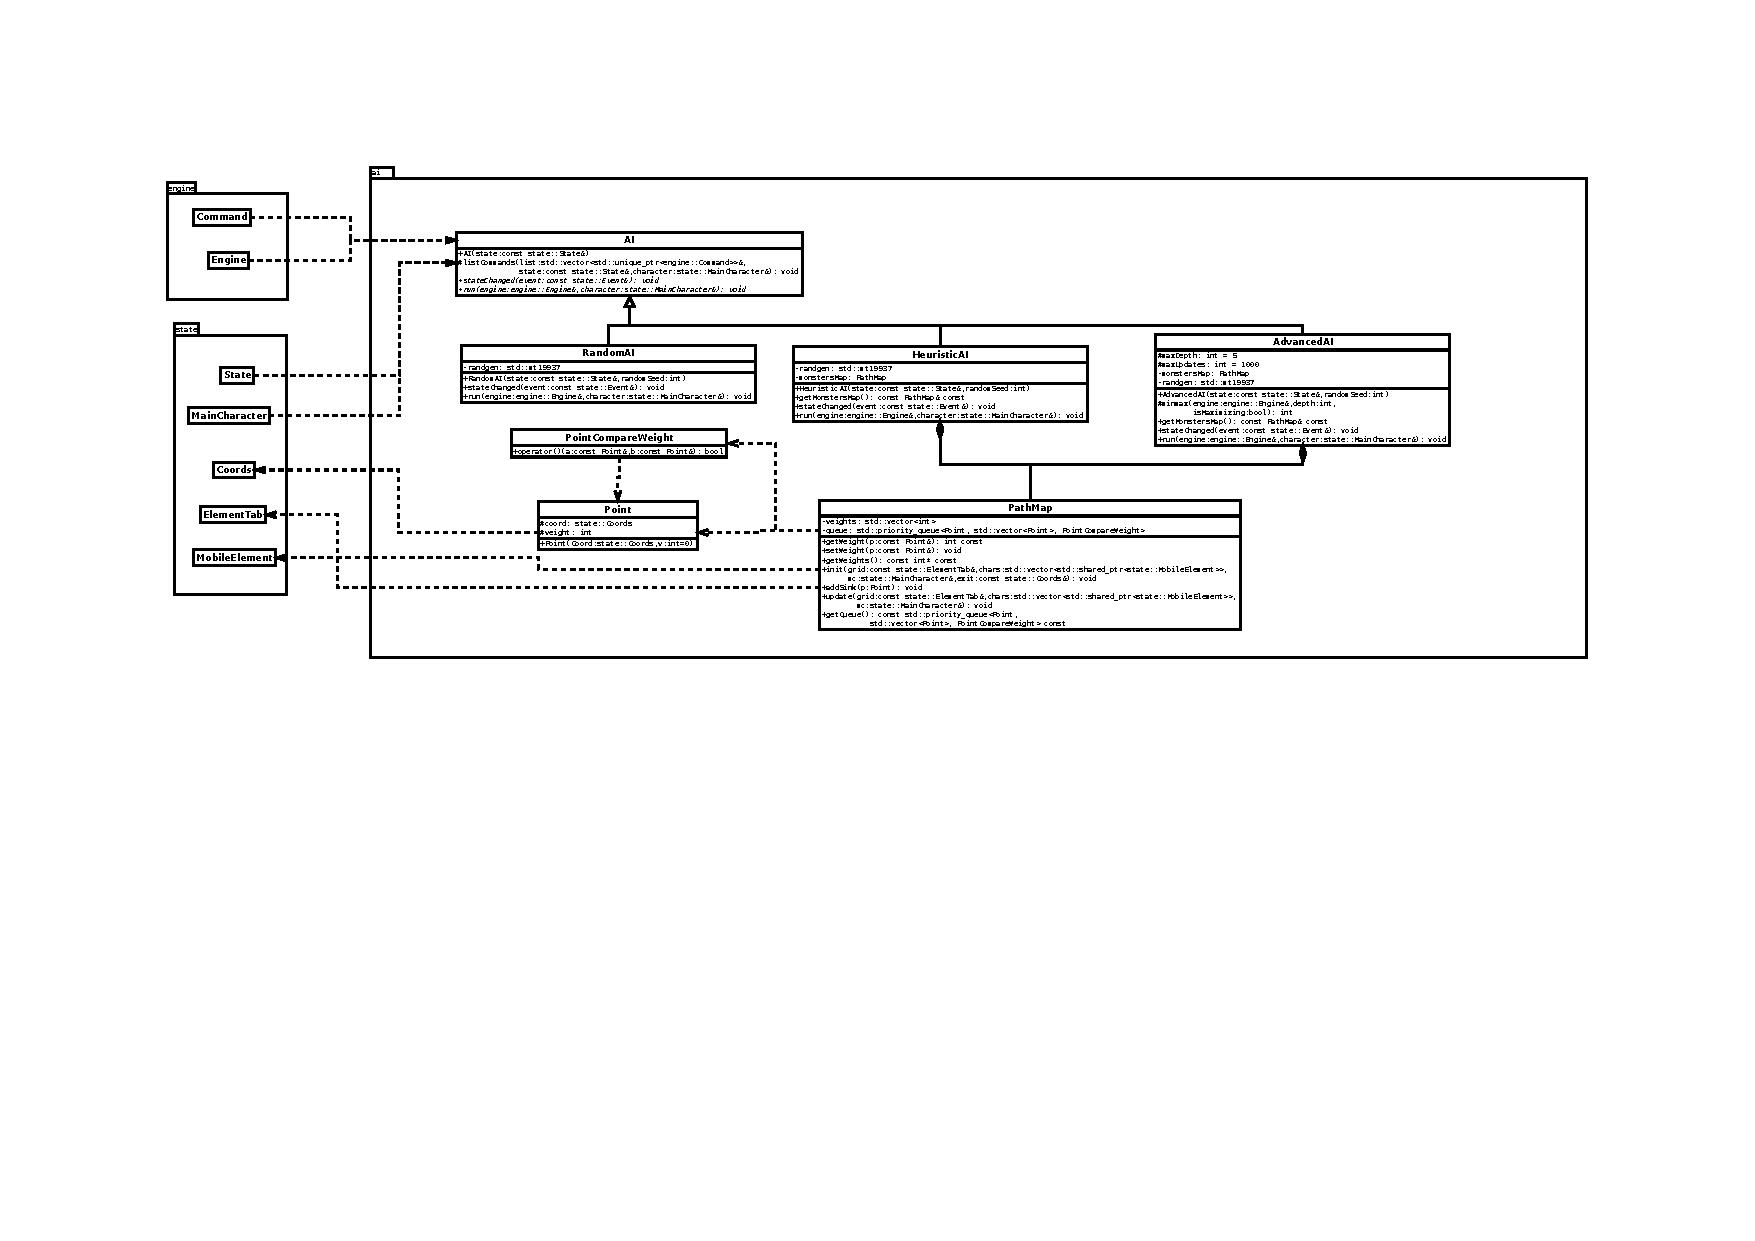
\includegraphics[width=0.9\paperheight]{ai.pdf}
%%\caption{\label{uml:ai}Diagramme des classes d'intelligence artificielle.} 
%%\end{figure}
%%\end{landscape}
%
%
%\section{Modularisation}
%\label{sec:module}
%
%\subsection{Organisation des modules}
%
%\clearpage
%\subsection{Conception logiciel}


%
%\begin{landscape}
%\begin{figure}[p]
%\includegraphics[width=0.9\paperheight]{module.pdf}
%\caption{\label{uml:module}Diagramme des classes pour la modularisation.} 
%\end{figure}
%\end{landscape}
 \addcontentsline{toc}{section}{Sources}
\section*{Sources}

\begin{itemize}
\item[Tiles :] DungeonTiles II \href{https://0x72.itch.io/dungeontileset-ii}{https://0x72.itch.io/dungeontileset-ii} par 0x72
\item[Font :] Pixel Font \href{https://devilsworkshop.itch.io/pixel-font}{https://devilsworkshop.itch.io/pixel-font


} par Ajay Karat | Devil's Work.shop
\end{itemize}

\end{document}
